% Created by tikzDevice version 0.12.3.2 on 2022-02-18 16:26:58
% !TEX encoding = UTF-8 Unicode
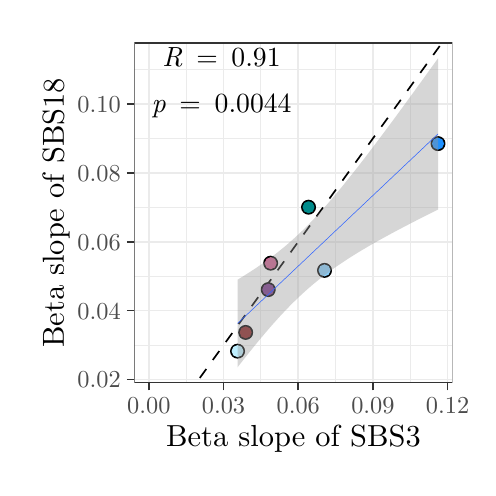
\begin{tikzpicture}[x=1pt,y=1pt]
\definecolor{fillColor}{RGB}{255,255,255}
\path[use as bounding box,fill=fillColor,fill opacity=0.00] (0,0) rectangle (158.99,158.99);
\begin{scope}
\path[clip] (  0.00,  0.00) rectangle (158.99,158.99);
\definecolor{drawColor}{RGB}{255,255,255}
\definecolor{fillColor}{RGB}{255,255,255}

\path[draw=drawColor,line width= 0.6pt,line join=round,line cap=round,fill=fillColor] (  0.00,  0.00) rectangle (158.99,158.99);
\end{scope}
\begin{scope}
\path[clip] ( 38.56, 30.69) rectangle (153.49,153.49);
\definecolor{fillColor}{RGB}{255,255,255}

\path[fill=fillColor] ( 38.56, 30.69) rectangle (153.49,153.49);
\definecolor{drawColor}{gray}{0.92}

\path[draw=drawColor,line width= 0.3pt,line join=round] ( 38.56, 44.28) --
	(153.49, 44.28);

\path[draw=drawColor,line width= 0.3pt,line join=round] ( 38.56, 69.18) --
	(153.49, 69.18);

\path[draw=drawColor,line width= 0.3pt,line join=round] ( 38.56, 94.08) --
	(153.49, 94.08);

\path[draw=drawColor,line width= 0.3pt,line join=round] ( 38.56,118.98) --
	(153.49,118.98);

\path[draw=drawColor,line width= 0.3pt,line join=round] ( 38.56,143.88) --
	(153.49,143.88);

\path[draw=drawColor,line width= 0.3pt,line join=round] ( 57.28, 30.69) --
	( 57.28,153.49);

\path[draw=drawColor,line width= 0.3pt,line join=round] ( 84.27, 30.69) --
	( 84.27,153.49);

\path[draw=drawColor,line width= 0.3pt,line join=round] (111.26, 30.69) --
	(111.26,153.49);

\path[draw=drawColor,line width= 0.3pt,line join=round] (138.26, 30.69) --
	(138.26,153.49);

\path[draw=drawColor,line width= 0.6pt,line join=round] ( 38.56, 31.83) --
	(153.49, 31.83);

\path[draw=drawColor,line width= 0.6pt,line join=round] ( 38.56, 56.73) --
	(153.49, 56.73);

\path[draw=drawColor,line width= 0.6pt,line join=round] ( 38.56, 81.63) --
	(153.49, 81.63);

\path[draw=drawColor,line width= 0.6pt,line join=round] ( 38.56,106.53) --
	(153.49,106.53);

\path[draw=drawColor,line width= 0.6pt,line join=round] ( 38.56,131.43) --
	(153.49,131.43);

\path[draw=drawColor,line width= 0.6pt,line join=round] ( 43.78, 30.69) --
	( 43.78,153.49);

\path[draw=drawColor,line width= 0.6pt,line join=round] ( 70.77, 30.69) --
	( 70.77,153.49);

\path[draw=drawColor,line width= 0.6pt,line join=round] ( 97.77, 30.69) --
	( 97.77,153.49);

\path[draw=drawColor,line width= 0.6pt,line join=round] (124.76, 30.69) --
	(124.76,153.49);

\path[draw=drawColor,line width= 0.6pt,line join=round] (151.75, 30.69) --
	(151.75,153.49);
\definecolor{drawColor}{RGB}{0,0,0}

\path[draw=drawColor,line width= 0.6pt,dash pattern=on 4pt off 4pt ,line join=round] ( 38.77,  0.00) -- (153.68,158.99);
\definecolor{fillColor}{RGB}{0,0,0}

\path[draw=drawColor,line width= 0.4pt,line join=round,line cap=round,fill=fillColor] ( 87.81, 73.89) circle (  2.50);

\path[draw=drawColor,line width= 0.4pt,line join=round,line cap=round,fill=fillColor] (148.27,117.10) circle (  2.50);

\path[draw=drawColor,line width= 0.4pt,line join=round,line cap=round,fill=fillColor] ( 78.77, 48.87) circle (  2.50);

\path[draw=drawColor,line width= 0.4pt,line join=round,line cap=round,fill=fillColor] (101.49, 94.12) circle (  2.50);

\path[draw=drawColor,line width= 0.4pt,line join=round,line cap=round,fill=fillColor] ( 86.93, 64.34) circle (  2.50);

\path[draw=drawColor,line width= 0.4pt,line join=round,line cap=round,fill=fillColor] (107.26, 71.29) circle (  2.50);

\path[draw=drawColor,line width= 0.4pt,line join=round,line cap=round,fill=fillColor] ( 75.84, 42.10) circle (  2.50);
\definecolor{drawColor}{RGB}{205,96,144}
\definecolor{fillColor}{RGB}{205,96,144}

\path[draw=drawColor,line width= 0.4pt,line join=round,line cap=round,fill=fillColor] ( 87.81, 73.89) circle (  1.96);
\definecolor{drawColor}{RGB}{30,144,255}
\definecolor{fillColor}{RGB}{30,144,255}

\path[draw=drawColor,line width= 0.4pt,line join=round,line cap=round,fill=fillColor] (148.27,117.10) circle (  1.96);
\definecolor{drawColor}{RGB}{139,35,35}
\definecolor{fillColor}{RGB}{139,35,35}

\path[draw=drawColor,line width= 0.4pt,line join=round,line cap=round,fill=fillColor] ( 78.77, 48.87) circle (  1.96);
\definecolor{drawColor}{RGB}{0,139,139}
\definecolor{fillColor}{RGB}{0,139,139}

\path[draw=drawColor,line width= 0.4pt,line join=round,line cap=round,fill=fillColor] (101.49, 94.12) circle (  1.96);
\definecolor{drawColor}{RGB}{122,55,139}
\definecolor{fillColor}{RGB}{122,55,139}

\path[draw=drawColor,line width= 0.4pt,line join=round,line cap=round,fill=fillColor] ( 86.93, 64.34) circle (  1.96);
\definecolor{drawColor}{RGB}{135,206,250}
\definecolor{fillColor}{RGB}{135,206,250}

\path[draw=drawColor,line width= 0.4pt,line join=round,line cap=round,fill=fillColor] (107.26, 71.29) circle (  1.96);
\definecolor{drawColor}{RGB}{191,239,255}
\definecolor{fillColor}{RGB}{191,239,255}

\path[draw=drawColor,line width= 0.4pt,line join=round,line cap=round,fill=fillColor] ( 75.84, 42.10) circle (  1.96);
\definecolor{fillColor}{RGB}{153,153,153}

\path[fill=fillColor,fill opacity=0.40] ( 75.84, 67.92) --
	( 76.75, 68.48) --
	( 77.67, 69.04) --
	( 78.59, 69.61) --
	( 79.50, 70.19) --
	( 80.42, 70.77) --
	( 81.34, 71.37) --
	( 82.26, 71.98) --
	( 83.17, 72.59) --
	( 84.09, 73.22) --
	( 85.01, 73.85) --
	( 85.92, 74.50) --
	( 86.84, 75.17) --
	( 87.76, 75.84) --
	( 88.67, 76.53) --
	( 89.59, 77.23) --
	( 90.51, 77.95) --
	( 91.42, 78.69) --
	( 92.34, 79.43) --
	( 93.26, 80.20) --
	( 94.17, 80.98) --
	( 95.09, 81.78) --
	( 96.01, 82.60) --
	( 96.92, 83.44) --
	( 97.84, 84.29) --
	( 98.76, 85.16) --
	( 99.68, 86.05) --
	(100.59, 86.96) --
	(101.51, 87.89) --
	(102.43, 88.83) --
	(103.34, 89.79) --
	(104.26, 90.77) --
	(105.18, 91.76) --
	(106.09, 92.77) --
	(107.01, 93.79) --
	(107.93, 94.83) --
	(108.84, 95.88) --
	(109.76, 96.95) --
	(110.68, 98.03) --
	(111.59, 99.12) --
	(112.51,100.22) --
	(113.43,101.34) --
	(114.35,102.46) --
	(115.26,103.59) --
	(116.18,104.74) --
	(117.10,105.89) --
	(118.01,107.05) --
	(118.93,108.22) --
	(119.85,109.39) --
	(120.76,110.57) --
	(121.68,111.76) --
	(122.60,112.96) --
	(123.51,114.16) --
	(124.43,115.36) --
	(125.35,116.58) --
	(126.26,117.79) --
	(127.18,119.01) --
	(128.10,120.24) --
	(129.02,121.47) --
	(129.93,122.70) --
	(130.85,123.93) --
	(131.77,125.17) --
	(132.68,126.42) --
	(133.60,127.66) --
	(134.52,128.91) --
	(135.43,130.16) --
	(136.35,131.42) --
	(137.27,132.68) --
	(138.18,133.94) --
	(139.10,135.20) --
	(140.02,136.46) --
	(140.93,137.73) --
	(141.85,138.99) --
	(142.77,140.26) --
	(143.69,141.53) --
	(144.60,142.81) --
	(145.52,144.08) --
	(146.44,145.36) --
	(147.35,146.63) --
	(148.27,147.91) --
	(148.27, 93.26) --
	(147.35, 92.81) --
	(146.44, 92.35) --
	(145.52, 91.89) --
	(144.60, 91.43) --
	(143.69, 90.97) --
	(142.77, 90.51) --
	(141.85, 90.04) --
	(140.93, 89.58) --
	(140.02, 89.11) --
	(139.10, 88.64) --
	(138.18, 88.16) --
	(137.27, 87.69) --
	(136.35, 87.21) --
	(135.43, 86.73) --
	(134.52, 86.25) --
	(133.60, 85.77) --
	(132.68, 85.28) --
	(131.77, 84.79) --
	(130.85, 84.29) --
	(129.93, 83.79) --
	(129.02, 83.29) --
	(128.10, 82.79) --
	(127.18, 82.28) --
	(126.26, 81.77) --
	(125.35, 81.25) --
	(124.43, 80.73) --
	(123.51, 80.20) --
	(122.60, 79.66) --
	(121.68, 79.12) --
	(120.76, 78.58) --
	(119.85, 78.03) --
	(118.93, 77.47) --
	(118.01, 76.90) --
	(117.10, 76.33) --
	(116.18, 75.75) --
	(115.26, 75.16) --
	(114.35, 74.55) --
	(113.43, 73.94) --
	(112.51, 73.32) --
	(111.59, 72.69) --
	(110.68, 72.05) --
	(109.76, 71.39) --
	(108.84, 70.73) --
	(107.93, 70.05) --
	(107.01, 69.35) --
	(106.09, 68.64) --
	(105.18, 67.92) --
	(104.26, 67.17) --
	(103.34, 66.42) --
	(102.43, 65.64) --
	(101.51, 64.85) --
	(100.59, 64.04) --
	( 99.68, 63.22) --
	( 98.76, 62.37) --
	( 97.84, 61.51) --
	( 96.92, 60.63) --
	( 96.01, 59.73) --
	( 95.09, 58.82) --
	( 94.17, 57.88) --
	( 93.26, 56.93) --
	( 92.34, 55.96) --
	( 91.42, 54.98) --
	( 90.51, 53.98) --
	( 89.59, 52.96) --
	( 88.67, 51.93) --
	( 87.76, 50.89) --
	( 86.84, 49.83) --
	( 85.92, 48.76) --
	( 85.01, 47.67) --
	( 84.09, 46.58) --
	( 83.17, 45.47) --
	( 82.26, 44.35) --
	( 81.34, 43.22) --
	( 80.42, 42.08) --
	( 79.50, 40.94) --
	( 78.59, 39.78) --
	( 77.67, 38.62) --
	( 76.75, 37.45) --
	( 75.84, 36.27) --
	cycle;

\path[] ( 75.84, 67.92) --
	( 76.75, 68.48) --
	( 77.67, 69.04) --
	( 78.59, 69.61) --
	( 79.50, 70.19) --
	( 80.42, 70.77) --
	( 81.34, 71.37) --
	( 82.26, 71.98) --
	( 83.17, 72.59) --
	( 84.09, 73.22) --
	( 85.01, 73.85) --
	( 85.92, 74.50) --
	( 86.84, 75.17) --
	( 87.76, 75.84) --
	( 88.67, 76.53) --
	( 89.59, 77.23) --
	( 90.51, 77.95) --
	( 91.42, 78.69) --
	( 92.34, 79.43) --
	( 93.26, 80.20) --
	( 94.17, 80.98) --
	( 95.09, 81.78) --
	( 96.01, 82.60) --
	( 96.92, 83.44) --
	( 97.84, 84.29) --
	( 98.76, 85.16) --
	( 99.68, 86.05) --
	(100.59, 86.96) --
	(101.51, 87.89) --
	(102.43, 88.83) --
	(103.34, 89.79) --
	(104.26, 90.77) --
	(105.18, 91.76) --
	(106.09, 92.77) --
	(107.01, 93.79) --
	(107.93, 94.83) --
	(108.84, 95.88) --
	(109.76, 96.95) --
	(110.68, 98.03) --
	(111.59, 99.12) --
	(112.51,100.22) --
	(113.43,101.34) --
	(114.35,102.46) --
	(115.26,103.59) --
	(116.18,104.74) --
	(117.10,105.89) --
	(118.01,107.05) --
	(118.93,108.22) --
	(119.85,109.39) --
	(120.76,110.57) --
	(121.68,111.76) --
	(122.60,112.96) --
	(123.51,114.16) --
	(124.43,115.36) --
	(125.35,116.58) --
	(126.26,117.79) --
	(127.18,119.01) --
	(128.10,120.24) --
	(129.02,121.47) --
	(129.93,122.70) --
	(130.85,123.93) --
	(131.77,125.17) --
	(132.68,126.42) --
	(133.60,127.66) --
	(134.52,128.91) --
	(135.43,130.16) --
	(136.35,131.42) --
	(137.27,132.68) --
	(138.18,133.94) --
	(139.10,135.20) --
	(140.02,136.46) --
	(140.93,137.73) --
	(141.85,138.99) --
	(142.77,140.26) --
	(143.69,141.53) --
	(144.60,142.81) --
	(145.52,144.08) --
	(146.44,145.36) --
	(147.35,146.63) --
	(148.27,147.91);

\path[] (148.27, 93.26) --
	(147.35, 92.81) --
	(146.44, 92.35) --
	(145.52, 91.89) --
	(144.60, 91.43) --
	(143.69, 90.97) --
	(142.77, 90.51) --
	(141.85, 90.04) --
	(140.93, 89.58) --
	(140.02, 89.11) --
	(139.10, 88.64) --
	(138.18, 88.16) --
	(137.27, 87.69) --
	(136.35, 87.21) --
	(135.43, 86.73) --
	(134.52, 86.25) --
	(133.60, 85.77) --
	(132.68, 85.28) --
	(131.77, 84.79) --
	(130.85, 84.29) --
	(129.93, 83.79) --
	(129.02, 83.29) --
	(128.10, 82.79) --
	(127.18, 82.28) --
	(126.26, 81.77) --
	(125.35, 81.25) --
	(124.43, 80.73) --
	(123.51, 80.20) --
	(122.60, 79.66) --
	(121.68, 79.12) --
	(120.76, 78.58) --
	(119.85, 78.03) --
	(118.93, 77.47) --
	(118.01, 76.90) --
	(117.10, 76.33) --
	(116.18, 75.75) --
	(115.26, 75.16) --
	(114.35, 74.55) --
	(113.43, 73.94) --
	(112.51, 73.32) --
	(111.59, 72.69) --
	(110.68, 72.05) --
	(109.76, 71.39) --
	(108.84, 70.73) --
	(107.93, 70.05) --
	(107.01, 69.35) --
	(106.09, 68.64) --
	(105.18, 67.92) --
	(104.26, 67.17) --
	(103.34, 66.42) --
	(102.43, 65.64) --
	(101.51, 64.85) --
	(100.59, 64.04) --
	( 99.68, 63.22) --
	( 98.76, 62.37) --
	( 97.84, 61.51) --
	( 96.92, 60.63) --
	( 96.01, 59.73) --
	( 95.09, 58.82) --
	( 94.17, 57.88) --
	( 93.26, 56.93) --
	( 92.34, 55.96) --
	( 91.42, 54.98) --
	( 90.51, 53.98) --
	( 89.59, 52.96) --
	( 88.67, 51.93) --
	( 87.76, 50.89) --
	( 86.84, 49.83) --
	( 85.92, 48.76) --
	( 85.01, 47.67) --
	( 84.09, 46.58) --
	( 83.17, 45.47) --
	( 82.26, 44.35) --
	( 81.34, 43.22) --
	( 80.42, 42.08) --
	( 79.50, 40.94) --
	( 78.59, 39.78) --
	( 77.67, 38.62) --
	( 76.75, 37.45) --
	( 75.84, 36.27);
\definecolor{drawColor}{RGB}{51,102,255}

\path[draw=drawColor,line width= 0.2pt,line join=round] ( 75.84, 52.09) --
	( 76.75, 52.96) --
	( 77.67, 53.83) --
	( 78.59, 54.69) --
	( 79.50, 55.56) --
	( 80.42, 56.43) --
	( 81.34, 57.30) --
	( 82.26, 58.16) --
	( 83.17, 59.03) --
	( 84.09, 59.90) --
	( 85.01, 60.76) --
	( 85.92, 61.63) --
	( 86.84, 62.50) --
	( 87.76, 63.36) --
	( 88.67, 64.23) --
	( 89.59, 65.10) --
	( 90.51, 65.97) --
	( 91.42, 66.83) --
	( 92.34, 67.70) --
	( 93.26, 68.57) --
	( 94.17, 69.43) --
	( 95.09, 70.30) --
	( 96.01, 71.17) --
	( 96.92, 72.03) --
	( 97.84, 72.90) --
	( 98.76, 73.77) --
	( 99.68, 74.64) --
	(100.59, 75.50) --
	(101.51, 76.37) --
	(102.43, 77.24) --
	(103.34, 78.10) --
	(104.26, 78.97) --
	(105.18, 79.84) --
	(106.09, 80.70) --
	(107.01, 81.57) --
	(107.93, 82.44) --
	(108.84, 83.31) --
	(109.76, 84.17) --
	(110.68, 85.04) --
	(111.59, 85.91) --
	(112.51, 86.77) --
	(113.43, 87.64) --
	(114.35, 88.51) --
	(115.26, 89.37) --
	(116.18, 90.24) --
	(117.10, 91.11) --
	(118.01, 91.98) --
	(118.93, 92.84) --
	(119.85, 93.71) --
	(120.76, 94.58) --
	(121.68, 95.44) --
	(122.60, 96.31) --
	(123.51, 97.18) --
	(124.43, 98.04) --
	(125.35, 98.91) --
	(126.26, 99.78) --
	(127.18,100.65) --
	(128.10,101.51) --
	(129.02,102.38) --
	(129.93,103.25) --
	(130.85,104.11) --
	(131.77,104.98) --
	(132.68,105.85) --
	(133.60,106.71) --
	(134.52,107.58) --
	(135.43,108.45) --
	(136.35,109.32) --
	(137.27,110.18) --
	(138.18,111.05) --
	(139.10,111.92) --
	(140.02,112.78) --
	(140.93,113.65) --
	(141.85,114.52) --
	(142.77,115.38) --
	(143.69,116.25) --
	(144.60,117.12) --
	(145.52,117.99) --
	(146.44,118.85) --
	(147.35,119.72) --
	(148.27,120.59);
\definecolor{drawColor}{RGB}{0,0,0}

\node[text=drawColor,anchor=base west,inner sep=0pt, outer sep=0pt, scale=  1.00] at ( 48.68,145.07) {\itshape R};

\node[text=drawColor,anchor=base west,inner sep=0pt, outer sep=0pt, scale=  1.00] at ( 55.94,145.07) { };

\node[text=drawColor,anchor=base west,inner sep=0pt, outer sep=0pt, scale=  1.00] at ( 60.92,145.07) {=};

\node[text=drawColor,anchor=base west,inner sep=0pt, outer sep=0pt, scale=  1.00] at ( 68.66,145.07) { };

\node[text=drawColor,anchor=base west,inner sep=0pt, outer sep=0pt, scale=  1.00] at ( 73.64,145.07) {0.91};

\node[text=drawColor,anchor=base west,inner sep=0pt, outer sep=0pt, scale=  1.00] at ( 44.79,128.24) {\itshape p};

\node[text=drawColor,anchor=base west,inner sep=0pt, outer sep=0pt, scale=  1.00] at ( 49.88,128.24) { };

\node[text=drawColor,anchor=base west,inner sep=0pt, outer sep=0pt, scale=  1.00] at ( 54.85,128.24) {=};

\node[text=drawColor,anchor=base west,inner sep=0pt, outer sep=0pt, scale=  1.00] at ( 62.60,128.24) { };

\node[text=drawColor,anchor=base west,inner sep=0pt, outer sep=0pt, scale=  1.00] at ( 67.58,128.24) {0.0044};
\definecolor{drawColor}{gray}{0.20}

\path[draw=drawColor,line width= 0.6pt,line join=round,line cap=round] ( 38.56, 30.69) rectangle (153.49,153.49);
\end{scope}
\begin{scope}
\path[clip] (  0.00,  0.00) rectangle (158.99,158.99);
\definecolor{drawColor}{gray}{0.30}

\node[text=drawColor,anchor=base east,inner sep=0pt, outer sep=0pt, scale=  0.88] at ( 33.61, 28.80) {0.02};

\node[text=drawColor,anchor=base east,inner sep=0pt, outer sep=0pt, scale=  0.88] at ( 33.61, 53.70) {0.04};

\node[text=drawColor,anchor=base east,inner sep=0pt, outer sep=0pt, scale=  0.88] at ( 33.61, 78.60) {0.06};

\node[text=drawColor,anchor=base east,inner sep=0pt, outer sep=0pt, scale=  0.88] at ( 33.61,103.50) {0.08};

\node[text=drawColor,anchor=base east,inner sep=0pt, outer sep=0pt, scale=  0.88] at ( 33.61,128.40) {0.10};
\end{scope}
\begin{scope}
\path[clip] (  0.00,  0.00) rectangle (158.99,158.99);
\definecolor{drawColor}{gray}{0.20}

\path[draw=drawColor,line width= 0.6pt,line join=round] ( 35.81, 31.83) --
	( 38.56, 31.83);

\path[draw=drawColor,line width= 0.6pt,line join=round] ( 35.81, 56.73) --
	( 38.56, 56.73);

\path[draw=drawColor,line width= 0.6pt,line join=round] ( 35.81, 81.63) --
	( 38.56, 81.63);

\path[draw=drawColor,line width= 0.6pt,line join=round] ( 35.81,106.53) --
	( 38.56,106.53);

\path[draw=drawColor,line width= 0.6pt,line join=round] ( 35.81,131.43) --
	( 38.56,131.43);
\end{scope}
\begin{scope}
\path[clip] (  0.00,  0.00) rectangle (158.99,158.99);
\definecolor{drawColor}{gray}{0.20}

\path[draw=drawColor,line width= 0.6pt,line join=round] ( 43.78, 27.94) --
	( 43.78, 30.69);

\path[draw=drawColor,line width= 0.6pt,line join=round] ( 70.77, 27.94) --
	( 70.77, 30.69);

\path[draw=drawColor,line width= 0.6pt,line join=round] ( 97.77, 27.94) --
	( 97.77, 30.69);

\path[draw=drawColor,line width= 0.6pt,line join=round] (124.76, 27.94) --
	(124.76, 30.69);

\path[draw=drawColor,line width= 0.6pt,line join=round] (151.75, 27.94) --
	(151.75, 30.69);
\end{scope}
\begin{scope}
\path[clip] (  0.00,  0.00) rectangle (158.99,158.99);
\definecolor{drawColor}{gray}{0.30}

\node[text=drawColor,anchor=base,inner sep=0pt, outer sep=0pt, scale=  0.88] at ( 43.78, 19.68) {0.00};

\node[text=drawColor,anchor=base,inner sep=0pt, outer sep=0pt, scale=  0.88] at ( 70.77, 19.68) {0.03};

\node[text=drawColor,anchor=base,inner sep=0pt, outer sep=0pt, scale=  0.88] at ( 97.77, 19.68) {0.06};

\node[text=drawColor,anchor=base,inner sep=0pt, outer sep=0pt, scale=  0.88] at (124.76, 19.68) {0.09};

\node[text=drawColor,anchor=base,inner sep=0pt, outer sep=0pt, scale=  0.88] at (151.75, 19.68) {0.12};
\end{scope}
\begin{scope}
\path[clip] (  0.00,  0.00) rectangle (158.99,158.99);
\definecolor{drawColor}{RGB}{0,0,0}

\node[text=drawColor,anchor=base,inner sep=0pt, outer sep=0pt, scale=  1.10] at ( 96.02,  7.64) {Beta slope of SBS3};
\end{scope}
\begin{scope}
\path[clip] (  0.00,  0.00) rectangle (158.99,158.99);
\definecolor{drawColor}{RGB}{0,0,0}

\node[text=drawColor,rotate= 90.00,anchor=base,inner sep=0pt, outer sep=0pt, scale=  1.10] at ( 13.08, 92.09) {Beta slope of SBS18};
\end{scope}
\end{tikzpicture}
